\chapter{The ecological niche concept}
\label{ch:TheEcologicalNicheConcept}
\section{Introduction}
\label{sec:chTheEcologicalNicheConcept:Introduction}
In this chapter the concept of the niche of a species is introduced. The ecological niche of a species can, non-rigorously, be defined as the set of environmental conditions where its reproduction rate is larger than or equal to its mortality rate. Although we will speak of the ecological niche, there are in fact at least three different ``definitions'' that are often used: the Grinnellian niche, the Eltonian niche, and the Hutchinsonian niche. Only a sketch of the niche concept will be given in this section. For a more rigorous description we refer the interested reader to \cite{soberon_grinnellian_2007, soberon_niches_2009}.

\section{Ecological versus geographical space}
In most databases that contain data about species only the location of a presence or absence record is available. Hence, these databases include information about the occurrences or absences in the so-called geographical space. Usually the range of a species' distribution is determined by environmental conditions. We will say that the corresponding variables span the environmental space. It is clear that for each point in the geographical space there is a point in the environmental space. This relation between environmental and geographical space is often called Hutchinson's duality \parencite{colwell_hutchinsons_2009}. A graphical representation of this relation is given in Figure \ref{fig:chTheEcologicalNicheConcept:Niche}. This duality relation is fundamental in SDMs, namely the predictors included in the model are usually assumed to be direct or indirect measures of the variables that span the environmental space. Once a model in the environmental space is constructed the duality relation allows us to make maps of the distribution in the geographical space. \\

\begin{figure}[!htb]
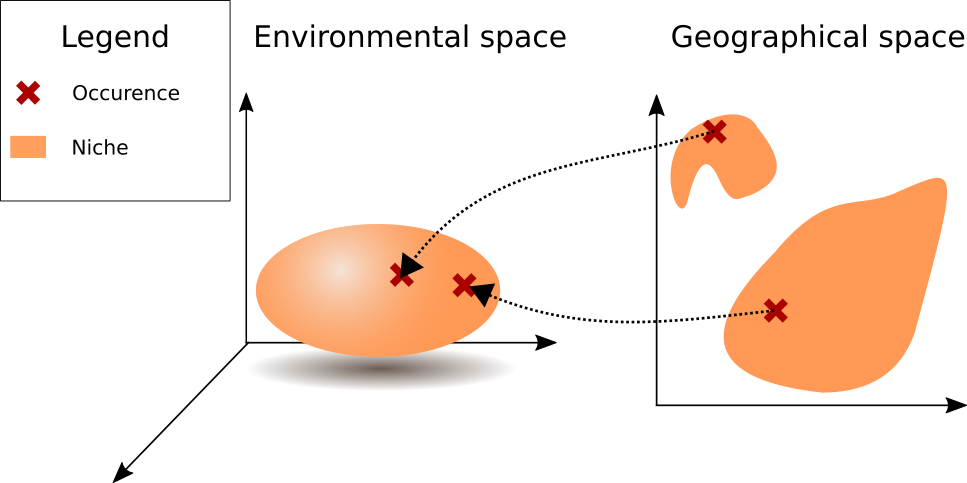
\includegraphics[scale=0.5]{VectorGraphics/Niche.png}
\caption{\label{fig:chTheEcologicalNicheConcept:Niche}Visualization of the duality between environmental and geographical space.}
\end{figure}

In practice a species will often not occur in certain parts of its niche. This can happen because of limited dispersal capabilities of the species, biotic interactions, etc. Such incomplete occupation of the niche leads to the concepts of a fundamental niche and the realized niche. The fundamental niche does not take into account whether or not the species is present, it only represents the suitable conditions. The realized niche is the subset of the fundamental niche where the species is present. These two concepts are depicted in Figure \ref{fig:chTheEcologicalNicheConcept:RealizedNiche}. 
\begin{figure}[!htb]
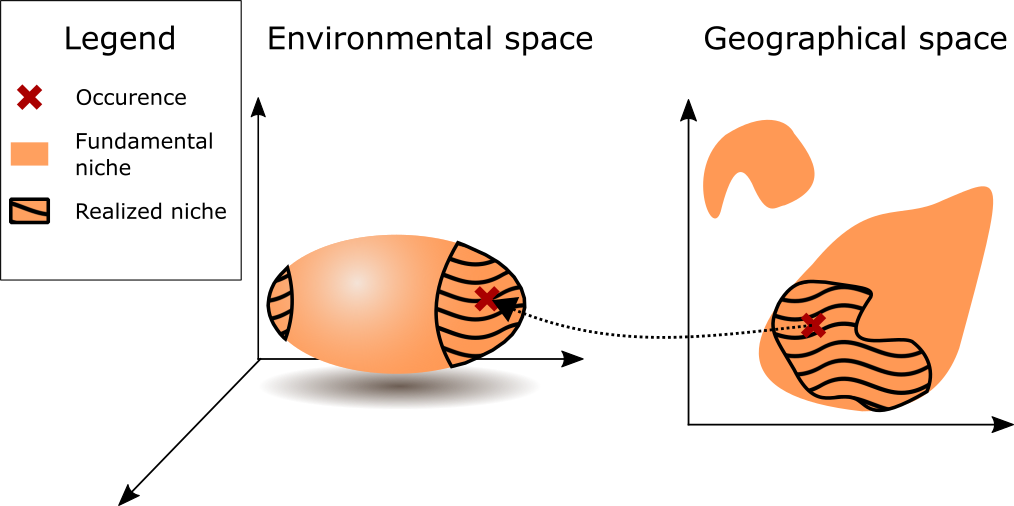
\includegraphics[scale=0.5]{VectorGraphics/RealizedNiche.png}
\caption{\label{fig:chTheEcologicalNicheConcept:RealizedNiche}Visualization of the difference between the fundamental and realized niche.}
\end{figure}

\section{Implicit assumptions when building and using species distribution modles}
\label{sec:chTheEcologicalNicheConcept:NicheEquilibrium}
Before applying SDMs in practice one has to realize that there are some important underlying assumptions. A few of these assumptions are described below. This is done in order to connect the theoretical niche concept to some more practical scenarios and to make the reader aware of the limitations of species distribution modelling. For a more complete overview of the underlying assumptions we refer to \cite{wiens_niches_2009}.\\

Every observed occurrence belongs, by definition, to the realized niche. SDMs are therefore models of the realized niche. If a SDM is used to e.g.\ predict areas prone to invasive species, it is implicitly assumed that, a part of, the realized niche is a good approximation of, a part of, the fundamental niche. Whether this assumption is realistic or not depends on: the species, whether the whole niche has to be approximated or only a part thereof, etc.\\

When data is used to build a model of the realized niche it is assumed that the observed data-points are representative of the niche. In practical settings this is often not the case. We give two examples:
\begin{enumerate}
\item Due to climate change tree species might be found in regions where the current environmental conditions are not included in its niche \parencite{woodward_impact_1990}.
\item The niche of a species usually evolves over time, therefore older observations might not be representative of the current niche \parencite{pearson_predicting_2003}.
\end{enumerate}

Another assumption that is implicitly made in most SDMs is that the effect of biotic interactions is negligible or indirectly captured by other environmental variables. However, in some applications explicitly including biotic interactions has been shown to improve the predictive capabilities \parencite[e.g.][]{heikkinen_biotic_2007}. \\


\section{Spatial scale}
\label{sec:SpatialScale}
From ecological theory we learn that the spatial scale and the extent of the study area play an important role in species distribution modelling \parencite{pearson_predicting_2003, pearson_modelling_2004}. \\

It is often argued that at large scales climate is the main driver of the distribution of species. Land-cover, soil type, and biotic interactions usually only become important when the climate is suitable and hence play a role in fine grain discrimination between suitable and unsuitable conditions. Furthermore, the role of the fine grain drivers might be influenced by the local climatic conditions. \\

The effect of the extent of the study area and the spatial scale are related. When a SDM is applied to a whole continent climate variables will make the biggest contribution to the model. If on the other hand a SDM is developed for a $10\times 10$ km area in Silkeborg the vegetation type might be more important than minor changes in climatic conditions.



